\documentclass[14pt]{extbook}
\usepackage{multicol, enumerate, enumitem, hyperref, color, soul, setspace, parskip, fancyhdr} %General Packages
\usepackage{amssymb, amsthm, amsmath, latexsym, units, mathtools} %Math Packages
\everymath{\displaystyle} %All math in Display Style
% Packages with additional options
\usepackage[headsep=0.5cm,headheight=12pt, left=1 in,right= 1 in,top= 1 in,bottom= 1 in]{geometry}
\usepackage[usenames,dvipsnames]{xcolor}
\usepackage{dashrule}  % Package to use the command below to create lines between items
\newcommand{\litem}[1]{\item#1\hspace*{-1cm}\rule{\textwidth}{0.4pt}}
\pagestyle{fancy}
\lhead{Progress Quiz 4}
\chead{}
\rhead{Version A}
\lfoot{5346-5907}
\cfoot{}
\rfoot{Summer C 2021}
\begin{document}

\begin{enumerate}
\litem{
Construct the lowest-degree polynomial given the zeros below. Then, choose the intervals that contain the coefficients of the polynomial in the form $ax^3+bx^2+cx+d$.\[ \frac{2}{3}, -7, \text{ and } \frac{7}{5} \]\begin{enumerate}[label=\Alph*.]
\item \( a \in [14, 16], b \in [74, 75], c \in [-204, -195], \text{ and } d \in [97, 102] \)
\item \( a \in [14, 16], b \in [74, 75], c \in [-204, -195], \text{ and } d \in [-98, -96] \)
\item \( a \in [14, 16], b \in [83, 101], c \in [-98, -83], \text{ and } d \in [-98, -96] \)
\item \( a \in [14, 16], b \in [-81, -66], c \in [-204, -195], \text{ and } d \in [-98, -96] \)
\item \( a \in [14, 16], b \in [-116, -113], c \in [62, 71], \text{ and } d \in [97, 102] \)

\end{enumerate} }
\litem{
Describe the zero behavior of the zero $x = 8$ of the polynomial below.\[ f(x) = -4(x + 8)^{7}(x - 8)^{10}(x - 4)^{4}(x + 4)^{8} \]\begin{enumerate}[label=\Alph*.]
\begin{multicols}{2}\item 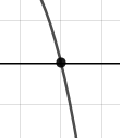
\includegraphics[width = 0.3\textwidth]{../Figures/polyZeroBehaviorAA.png}\item 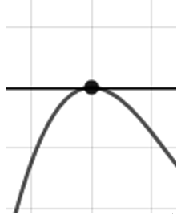
\includegraphics[width = 0.3\textwidth]{../Figures/polyZeroBehaviorBA.png}\item 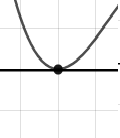
\includegraphics[width = 0.3\textwidth]{../Figures/polyZeroBehaviorCA.png}\item 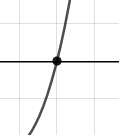
\includegraphics[width = 0.3\textwidth]{../Figures/polyZeroBehaviorDA.png}\end{multicols}\item None of the above.
\end{enumerate} }
\litem{
Construct the lowest-degree polynomial given the zeros below. Then, choose the intervals that contain the coefficients of the polynomial in the form $x^3+bx^2+cx+d$.\[ -2 + 4 i \text{ and } 4 \]\begin{enumerate}[label=\Alph*.]
\item \( b \in [0.9, 2.6], c \in [-10, -4.4], \text{ and } d \in [15, 18] \)
\item \( b \in [-3.1, 0.1], c \in [2.6, 4.7], \text{ and } d \in [79, 82] \)
\item \( b \in [0.9, 2.6], c \in [-6.7, 0.2], \text{ and } d \in [-12, -6] \)
\item \( b \in [-3.1, 0.1], c \in [2.6, 4.7], \text{ and } d \in [-82, -75] \)
\item \( \text{None of the above.} \)

\end{enumerate} }
\litem{
Which of the following equations \textit{could} be of the graph presented below?
\begin{center}
    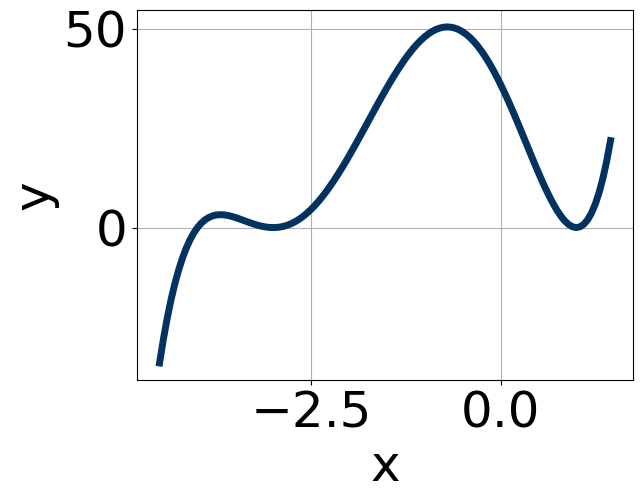
\includegraphics[width=0.5\textwidth]{../Figures/polyGraphToFunctionCopyA.png}
\end{center}
\begin{enumerate}[label=\Alph*.]
\item \( 3(x - 1)^{8} (x + 3)^{7} (x + 4)^{9} \)
\item \( 15(x - 1)^{4} (x + 3)^{8} (x + 4)^{5} \)
\item \( 13(x - 1)^{10} (x + 3)^{7} (x + 4)^{6} \)
\item \( -5(x - 1)^{6} (x + 3)^{4} (x + 4)^{4} \)
\item \( -11(x - 1)^{10} (x + 3)^{10} (x + 4)^{7} \)

\end{enumerate} }
\litem{
Describe the zero behavior of the zero $x = -5$ of the polynomial below.\[ f(x) = 6(x + 8)^{4}(x - 8)^{2}(x - 5)^{5}(x + 5)^{2} \]\begin{enumerate}[label=\Alph*.]
\begin{multicols}{2}\item 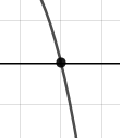
\includegraphics[width = 0.3\textwidth]{../Figures/polyZeroBehaviorCopyAA.png}\item 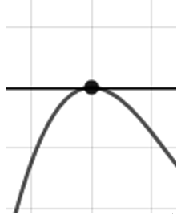
\includegraphics[width = 0.3\textwidth]{../Figures/polyZeroBehaviorCopyBA.png}\item 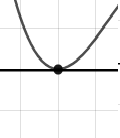
\includegraphics[width = 0.3\textwidth]{../Figures/polyZeroBehaviorCopyCA.png}\item 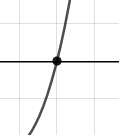
\includegraphics[width = 0.3\textwidth]{../Figures/polyZeroBehaviorCopyDA.png}\end{multicols}\item None of the above.
\end{enumerate} }
\litem{
Which of the following equations \textit{could} be of the graph presented below?
\begin{center}
    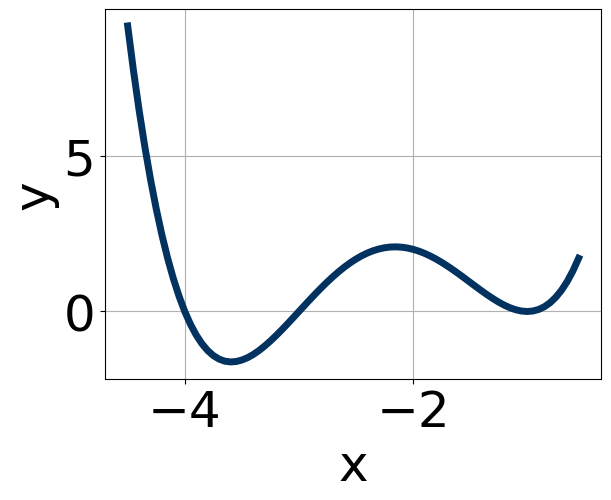
\includegraphics[width=0.5\textwidth]{../Figures/polyGraphToFunctionA.png}
\end{center}
\begin{enumerate}[label=\Alph*.]
\item \( -7(x + 1)^{6} (x + 3)^{9} (x + 4)^{7} \)
\item \( 3(x + 1)^{5} (x + 3)^{4} (x + 4)^{5} \)
\item \( 7(x + 1)^{8} (x + 3)^{9} (x + 4)^{11} \)
\item \( -7(x + 1)^{4} (x + 3)^{9} (x + 4)^{10} \)
\item \( 17(x + 1)^{6} (x + 3)^{8} (x + 4)^{5} \)

\end{enumerate} }
\litem{
Construct the lowest-degree polynomial given the zeros below. Then, choose the intervals that contain the coefficients of the polynomial in the form $x^3+bx^2+cx+d$.\[ 5 + 4 i \text{ and } 2 \]\begin{enumerate}[label=\Alph*.]
\item \( b \in [-20, -7], c \in [60, 64.2], \text{ and } d \in [-82.1, -78.6] \)
\item \( b \in [-4, 6], c \in [-9.6, -6.6], \text{ and } d \in [8.9, 14] \)
\item \( b \in [12, 16], c \in [60, 64.2], \text{ and } d \in [79, 82.4] \)
\item \( b \in [-4, 6], c \in [-6.7, -2.2], \text{ and } d \in [4.9, 9.8] \)
\item \( \text{None of the above.} \)

\end{enumerate} }
\litem{
Describe the end behavior of the polynomial below.\[ f(x) = 7(x + 8)^{4}(x - 8)^{7}(x + 3)^{3}(x - 3)^{3} \]\begin{enumerate}[label=\Alph*.]
\begin{multicols}{2}\item 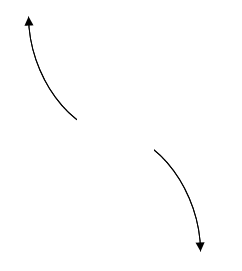
\includegraphics[width = 0.3\textwidth]{../Figures/polyEndBehaviorCopyAA.png}\item 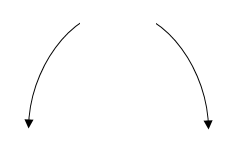
\includegraphics[width = 0.3\textwidth]{../Figures/polyEndBehaviorCopyBA.png}\item 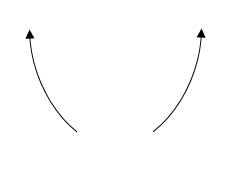
\includegraphics[width = 0.3\textwidth]{../Figures/polyEndBehaviorCopyCA.png}\item 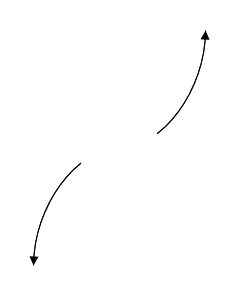
\includegraphics[width = 0.3\textwidth]{../Figures/polyEndBehaviorCopyDA.png}\end{multicols}\item None of the above.
\end{enumerate} }
\litem{
Describe the end behavior of the polynomial below.\[ f(x) = 5(x + 5)^{3}(x - 5)^{8}(x - 7)^{3}(x + 7)^{3} \]\begin{enumerate}[label=\Alph*.]
\begin{multicols}{2}\item 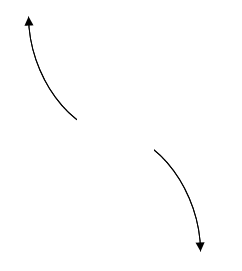
\includegraphics[width = 0.3\textwidth]{../Figures/polyEndBehaviorAA.png}\item 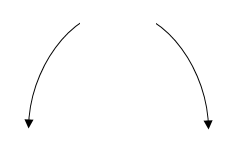
\includegraphics[width = 0.3\textwidth]{../Figures/polyEndBehaviorBA.png}\item 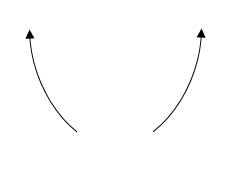
\includegraphics[width = 0.3\textwidth]{../Figures/polyEndBehaviorCA.png}\item 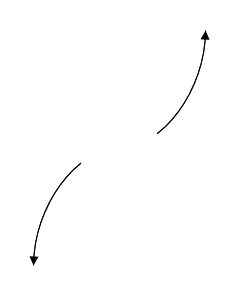
\includegraphics[width = 0.3\textwidth]{../Figures/polyEndBehaviorDA.png}\end{multicols}\item None of the above.
\end{enumerate} }
\litem{
Construct the lowest-degree polynomial given the zeros below. Then, choose the intervals that contain the coefficients of the polynomial in the form $ax^3+bx^2+cx+d$.\[ \frac{-3}{2}, \frac{-4}{3}, \text{ and } \frac{-1}{4} \]\begin{enumerate}[label=\Alph*.]
\item \( a \in [21, 26], b \in [2, 9], c \in [-61, -45], \text{ and } d \in [-12, -9] \)
\item \( a \in [21, 26], b \in [69, 75], c \in [60, 68], \text{ and } d \in [9, 16] \)
\item \( a \in [21, 26], b \in [-68, -61], c \in [27, 37], \text{ and } d \in [9, 16] \)
\item \( a \in [21, 26], b \in [69, 75], c \in [60, 68], \text{ and } d \in [-12, -9] \)
\item \( a \in [21, 26], b \in [-77, -65], c \in [60, 68], \text{ and } d \in [-12, -9] \)

\end{enumerate} }
\end{enumerate}

\end{document}